%=============================
%=============================
\subsection{Modèles de description \e{endogène}}\label{sec:insitu}
% \subsection{Descriptions métiers basées sur le plan}\label{sec:plan}
% Script, Storyboard (\cite{Martin2005}, \cite{ThiBui2003}) etc.


% Another trail of research has emerged recently. 
% In comparison to the previous approach, it does not attack the multimedia description from below (with signal processing techniques) but from above. 
% The principles is to represent the knowledge included in documents related to the multimedia content. 
% It can be a web-page where the image is published and commented by others \cite{Simperl2009} or more specific documents related to the production context. 
\e{
Des modèles de description, dit \e{endogène a priori}, sont apparus récemment avec pour approche de modéliser les connaissances contenues dans les documents de la chaîne de production audiovisuelle.
Nous présentons plus en détails un langage XML qui capture les informations contenus dans un script (\ref{sec:msml}) ainsi qu'un projet de recherche qui formalise une notation d'assistance aux réalisateurs à la direction de tournage, elle-même reposant sur le script (\ref{sec:answer}).}

\subsubsection{Movie Script Markup Langage}\label{sec:msml}
MSML est un modèle documentaire développé par \cite{VanRijsselbergen2009} qui permet de représenter des scripts pour la production télévisuelle et les films dramatiques. 
Le modèle se décompose en plusieurs parties, une partie décrivant le contenu, une autre sur la manière de fabriquer ce contenu et d'autres qui visent à fournir une pré-visualisation en 3D du contenu.
MSML est représenté en XML Schema et utilise Schematron \parcite{ISO/IEC2006} pour édicter des règles plus complexes de validation de la structure des documents XML construits.

\begin{figure}[ht!]
\centering
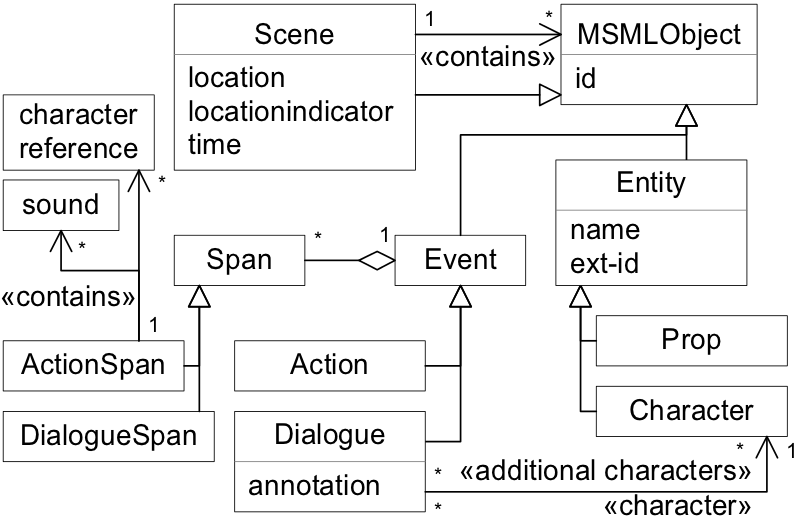
\includegraphics[width=0.6\textwidth]{images/MSML-sceneModel.png}
\caption{Modélisation d'un script audiovisuel en MSML}
\label{img:msml-model}
\end{figure}

% \paragraph{Modèle de scène}
MSML repose sur la \e{scène} en tant qu'unité narrative, dans laquelle se déroule des \e{évènements} dans un \e{lieu} et à un moment donné, c'est-à-dire un \e{intervalle continu de temps}, voir Figure \ref{img:msml-model}.
Des \e{entités} (éléments) sont présentes dans la \e{scène}, soit des \e{accessoires} qui décorent, soit des \e{personnages} qui participent à l'évolution de l'histoire.
Les \e{évènements} peuvent être décomposés en deux types, soit des \e{actions} qui représentent également la description d'une scène (cadre, environnement, ambiance etc.), soit des \e{dialogues} entre personnages.
La représentation des \e{évènements} peut être associée avec une représentation du temps écoulé, c'est-à-dire de sa \e{durée} (\pc{span}).
Les éléments de \e{durée} servent à combiner des évènements de nature différente, comme un dialogue et une action qui se réaliseraient  simultanément, ou bien une action qui donnerait des indications sur la manière de jouer le dialogue.


% \paragraph{Modèle de fabrication}
Le modèle de fabrication représente les \e{appareils techniques} (\pc{Component}) de captation, la \e{lumière} et le \e{plateau} afin de leur associer des \e{instructions}.
Ces \e{instructions} sont des annotations textuelles écrites librement par le réalisateur pour indiquer la manière de fabriquer le contenu.
Il peut s'agir par exemple, d'indiquer le type de plan souhaité par le réalisateur pour filmer un dialogue, pour réaliser la prise de son avec tel micro etc.

\begin{figure}[ht!]
\centering
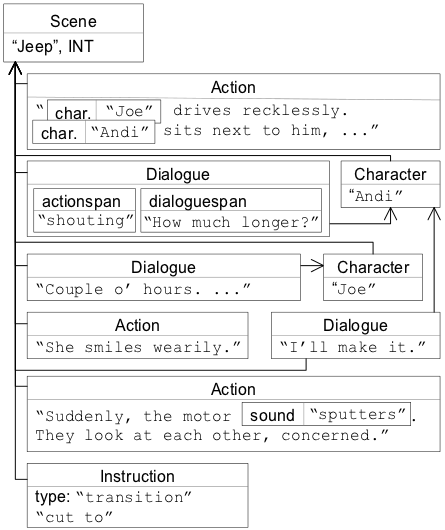
\includegraphics[width=0.6\textwidth]{images/MSML-sceneExample.png}
\caption{Exemple de représentation d'un script audiovisuel en MSML}
\label{img:msml-ex}
\end{figure}

La Figure \ref{img:msml-ex} montre un exemple de script décomposé selon les modèles de scène et de fabrication. 
La scène se déroule dans une Jeep, deux personnages, Andi et Joe sont assis l'un à côté de l'autre et parlent. 
La description de la scène est contenue dans un évènement \e{action}, puis Andi pose une question à Joe, représenté par un évènement \e{dialogue}. 
On voit ainsi comment est réalisé la composition des éléments dialogue et action par l'intermédiaire des \e{durées}.
L'action servant à décrire la manière dont le dialogue est énoncé par Andi.
La scène se termine par une \e{instruction} de type transition qui indique au monteur qu'il faudra directement passer au plan suivant sans faire de fondu entre les plans.


% \paragraph{Modèles de Pré-visualisation}
% A similar work has been carried out by \cite{VanRijsselbergen2009} but with distinct goal and language. 
% Their MovieScriptMarkupLanguage (MSML) captures the information of a shooting script with a particular attention to the details of set equipment's and actor's positions. 

En vue de proposer une pré-visualisation graphique des évènements décrits dans le script, MSML propose des éléments permettant d'affiner la représentation du temps, ainsi que des éléments de description des animations.
Il s'agit en particulier de préciser la succession et la synchronisation des \e{évènements} se déroulant dans le script. 
En effet, le texte du script décrit ces évènements ligne par ligne ce qui ne permet pas d'indiquer de relation temporelle entre eux.
Ainsi, ils peuvent très bien se produire en simultané, avec plus ou moins de temps entre eux etc.
De plus, les \e{animations} permettent de décomposer le mouvement d'une entité (objet, personnage) en plusieurs parties.

\paragraph{Discussion}
Le modèle MSML a été illustré dans l'application \pc{Scoop} développée par \cite{Cardinaels2008}. 
Il permet de coupler une représentation 3D d'un plateau et des personnages, avec la représentation du script et des équipements de production.
Ainsi, un réalisateur peut modifier l'emplacement d'une caméra sur le plateau et observer directement l'effet sur le plan filmé. 
L'objectif est de faciliter la préparation du tournage, notamment dans des environnements de plateau où la place est restreinte et le positionnement du décor difficile.
Les informations récoltées pourraient également être réutilisées plus tard dans la production, cependant la représentation de script en fichier XML pose un problème de transformation des données et d'interopérabilité avec les applications de fin de chaîne.
La synchronisation entre ces descriptions et le contenu filmé est également un problème qui n'est pas abordé par \cite{VanRijsselbergen2009}. 

Le positionnement de MSML sur les connaissances spécifiques à la pré-production en fait un modèle à part parmi les modélisations que nous étudions.
Son originalité provient de sa modélisation du contenu à produire selon un découpage narratif (scène), puis sur les indications de tournage dont il est possible d'observer les conséquences par l'intermédiaire d'une application.
Ce point de vue de description particulier tranche avec des modélisations qui se concentre sur le matériel audiovisuel [\g{$\chi_1$ : autonomie}] mais rend de ce fait difficile leur association [\g{$\chi_2$ : réutilisabilité}].


% The related  system  provides its user 3D model of the set as well as the shots taken by the camera in a given position and settings. 
% The overall objective is to provide an shooting-set 3D simulation to assist the production team in their preparation.\\



\subsubsection{Projet \pc{Answer}}\label{sec:answer}
Le projet \pc{Answer} est un projet financé par le 7ème PCRD qui instrumente la pratique de direction des réalisateurs de film \parcite{UniversityofSouthamptonITInnovation2009}. 
Les résultats du projet comportent des applications et une ontologie décomposées en plusieurs parties : 

\begin{figure}[ht!]
\centering
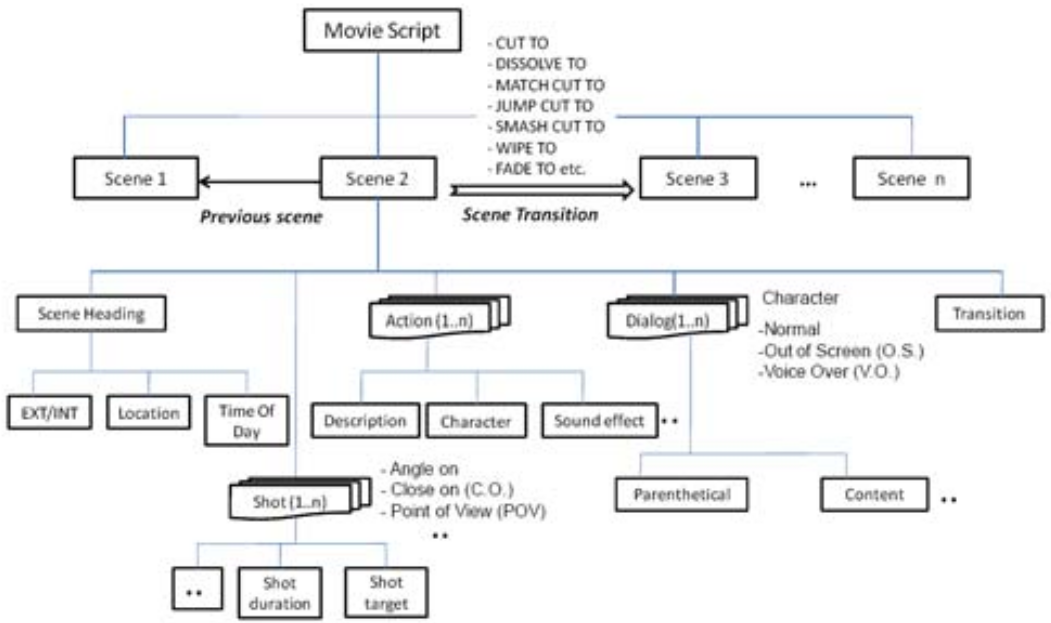
\includegraphics[width=\textwidth]{images/Ontofilm-concepts.png}
\caption{Modélisation d'un script audiovisuel dans \pc{Answer}}
\label{img:ontofilm}
\end{figure}

\begin{listeni}
	\item une \gpc{Context Ontology} qui modélise le processus de production d'un film, les équipements techniques de captation, les décors, les costumes ainsi que des règles de réalisation audiovisuelle (règles d'enchaînement de plans, caractéristiques de tournage des plans etc.).
	Par la suite, des éléments spécifiques au développement des jeux vidéos ont été rajouté à cette ontologie.
	Cette partie de l'ontologie comporte en particulier : 

	\begin{liste}
		\item un modèle de pré-production qui décompose un \e{script} en scènes et plans, voir Figure \ref{img:ontofilm} \parcite{Chakravarthy2009a}.
		Les scènes sont décrites par rapport aux personnages présents, aux actions se déroulant ou aux dialogues ainsi que les transitions, d'une manière très proche des scripts papiers.
		Le modèle a fait l'objet d'une représentation proche des formats des logiciels d'écriture de script professionnels.  
		Cette représentation est utilisée dans l'application \pc{Editor}, développée dans le cadre du projet, et qui permet aux réalisateurs d'annoter des scripts.\\
	\end{liste}

	\item une \gpc{Core Ontology} qui constitue un modèle de direction artistique également nommée \pc{Director Notation} \parcite{Chakravarthy2009b}. 
	Cette notation vise à préciser le jeu d'acteurs (position, émotion, mouvement etc.) pour chaque plan du script. 
	L'application \pc{Editor} permet d'écrire ces annotations à côté du script à partir d'une palette de symboles visuels. 
	Un service Web, le \pc{Rule Engine}, transforme ces symboles en des instances de l'ontologie représentant la géométrie du film et de la \gui{scène} filmée.
	Ces instances peuvent ensuite être utilisées par une application de pré-visualisation de la scène en 3D, avec animation des personnages etc.

	\item une intégration de concepts de MPEG-7 comme ontologie générique. 
	Il s'agit en particulier du Segment DS mais aussi de descripteurs plus spécifiques pour la couleur, la texture, les mouvements de caméra etc.
\end{listeni}

\paragraph{Discussion}
L'intérêt de cette modélisation est d'associer des connaissances sur la production, c'est-à-dire comment a été construit le film, et le résultat de cette production, le film en tant que tel [\g{$\chi_2$ : réutilisabilité}].
Ceci est rendu possible par le fait que la structure d'annotation est celle du script, qui correspond à la fois à une unité de contenu -- le film -- et une unité de travail pour la production [\g{$\chi_1$ : autonomie}].
Ce projet propose ainsi une approche de description intégrée aux pratiques et au vocabulaire de la production filmique, en instrumentant le travail de ses contributeurs.
Il est néanmoins regrettable que leurs résultats ne soient pas accessibles à la communauté scientifique, qu'il s'agisse des applications ou bien de l'ontologie, ce qui rend difficile la réutilisation de leurs travaux. 






%=============================
%=============================
% \subsection{Modèles et standards de description}
\subsection{Modèles de description \e{exogènes}}\label{sec:post}
\e{
Nous présentons d'abord le Dublin Core, un modèle de description à vocation générique qui peut s'appliquer à tous types de ressources sur le Web (\ref{sec:dcmi}).
Ensuite, nous introduisons plusieurs parties du standard MPEG-7 (\ref{sec:mpeg7}, \ref{sec:mpeg7-gc}, \ref{sec:mpeg7-dc}), et comparons des travaux de formalisation de ce standard qui visent à constituer une ontologie noyau pour le multimédia (\ref{sec:mpeg7etc}).
Enfin, nous présentons une proposition d'alignement minimaliste qui permet d'aggréger les informations représentées dans de multiples modèles multimédia (\ref{sec:omr}).}



\subsubsection{Dublin Core Metadata Initiative: Metadata Terms}\label{sec:dcmi}
\begin{table}[htb!]
   \begin{center}
		\begin{tabularx}{0.75\textwidth}{l X}
		   \hline
\gpc{Propriété} & \gpc{Sous-propriétés} \\ \hline
accrualMethod & \\ \hline
accrualPeriodicity & \\ \hline
accrualPolicy & \\ \hline
audience & 
	educationLevel, mediator\\ \hline
\e{contributor} & 
	\e{creator} \\ \hline
\e{coverage} & 
	spatial, temporal \\ \hline
\e{date} & 
	available, created, dateAccepted, dateCopyrighted, dateSubmitted, issued, modified,	valid  \\ \hline

\e{description} & 
	abstract, tableOfContents \\ \hline
\e{format} & 
	extent, medium \\ \hline
\e{identifier} & 
	bibliographicCitation \\ \hline

instructionalMethod & \\ \hline
\e{language} & \\ \hline
provenance & \\ \hline
\e{publisher} & \\ \hline
\e{relation} &
	conformsTo, hasFormat, hasPart, hasVersion, isFormatOf,	isPartOf, 	isReferencedBy, isReplacedBy, isRequiredBy, isVersionOf, references, replaces, requires, \e{source} \\ \hline 
\e{rights} & 
	accessRights, license \\ \hline
rightsHolder & \\ \hline
\e{subject} & \\ \hline
\e{title} & 
	alternative \\ \hline
\e{type} & \\ \hline
\end{tabularx}
\caption{Liste des propriétés et sous-propriétés du DCMI Metadata Terms}\label{tab:dcmi}
\end{center}
\end{table}

La \pc{Dublin Core Metadata Initiative} (DCMI) est une organisation qui vise à développer et promouvoir l'usage de standards de description de ressources afin de faciliter l'échange d'information sur le Web.
Depuis la première conférence organisée en 1995 à Dublin, Ohio, l'organisation a enrichi le vocabulaire de son standard original, le \pc{Dublic Core Metadata Element Set} (DCMES), de nouveaux éléments. 
En effet, la version étendue de \pc{DCMI Metadata Terms} (\cite{DCMIUsageBoard2010}) compte 54 propriétés et sous-propriétés, dont les 15 éléments d'origines (marqués en \e{italique} dans la Table \ref{tab:dcmi}).
L'intérêt de cette structuration est de pouvoir remplacer les valeurs des sous-propriétés comme des valeurs de leur propriété parente. 
La structuration des propriétés est telle que la valeur conserve une signification, même si celle-ci correspond à une propriété moins précise. 
Cela sert notamment pour réaliser des inférences et de l'enrichissement de requêtes.
Nous rappelons d'abord le modèle général du Dublin Core, puis nous présentons en particulier les Schémas d'encodage qui servent à détailler le champs de valeurs utilisable pour une propriété.
Enfin, nous discutons une proposition de spécialisation du Dublin Core pour couvrir spécifiquement la description de documents audiovisuels.

\begin{figure}[ht!]
\centering
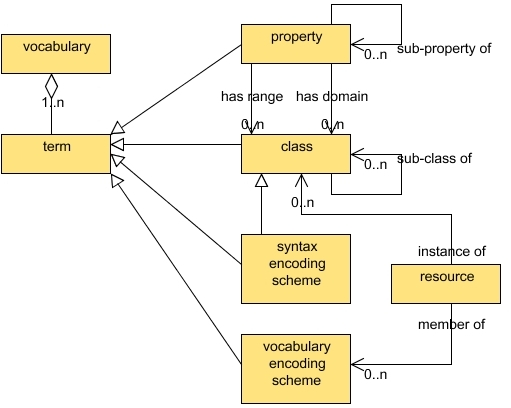
\includegraphics[width=0.6\textwidth]{images/vocabulary-model.jpg}
\caption{Modèle général du DCMI}
\label{img:dcmi-voc}
\end{figure}

\paragraph{Modèle général et représentation}
Une des grandes avancées de \pc{DCMI Metadata Terms}, a été la constitution d'une modélisation générale, voir la Figure \ref{img:dcmi-voc}, et l'introduction d'une syntaxe de représentation utilisant XML, RDF et RDF-S. 
En plus des propriétés, le modèle définit les notions de Classe et de Schéma d'encodage (qui seront expliquées ci-après). 
Les classes permettent de définir des types de ressources et de leur attribuer des URI. 

Chaque \pc{Terme} est défini par une liste d'attributs lui donnant un identifiant, une étiquette, une définition qui permet des commentaires, de la documentation, une référence complémentaire, les relations hiérarchiques avec les autres Termes, la classe et le type du Terme, l'appartenance à un Schéma d'encodage, les restrictions de sujet et d'objet qui s'applique à une propriété, les propriétés équivalentes.
Ainsi, on peut maintenant utiliser des URI, faisant référence à d'autres ressources, comme valeur d'une propriété.
Les valeurs peuvent donc être soit une expression littérale, une URI quelconque, ou bien une URI pointant vers un type de ressource particulier, comme un Terme appartenant à un schéma d'encodage ou une classe.
Par exemple, la propriété \pc{creator} ne peut pointer que vers des ressources de classe \pc{Agent} (du fait d'une restriction \pc{hasRange}). 


\paragraph{Schémas d'encodage}
Il existe deux types de schémas d'encodage qui permettent de préciser si les valeurs des propriétés sont écrites selon une syntaxe particulière (\pc{Syntax Encoding Scheme}, SES), ou si la valeur fait partie d'un thésaurus ou d'un vocabulaire contrôlé (\pc{Vocabulary Encoding Scheme}, VES).
Cela permet par exemple, d'indiquer que les valeurs de la propriété \pc{date} sont écrites suivant le format du W3C Date Time Format ou bien suivant la norme ISO 8106. 
De même, on peut déclarer que les valeurs de la propriété \pc{subject} seront prises dans la liste des \pc{Library of Congress Subject Headings}. 
%need REF ! 
SES et VES offrent ainsi la possibilité d'utiliser plusieurs jargons ou syntaxes pour caractériser les valeurs des propriétés, voir [$\delta_1$] dans les besoins de modélisations du chapitre précédent (\ref{sec:bm}).
De plus, la spécification d'un Terme permet d'ajouter une définition et de pointer vers d'autres ressources pour documenter les Termes, voir [$\delta_2$].

\begin{figure}[ht!]
\centering
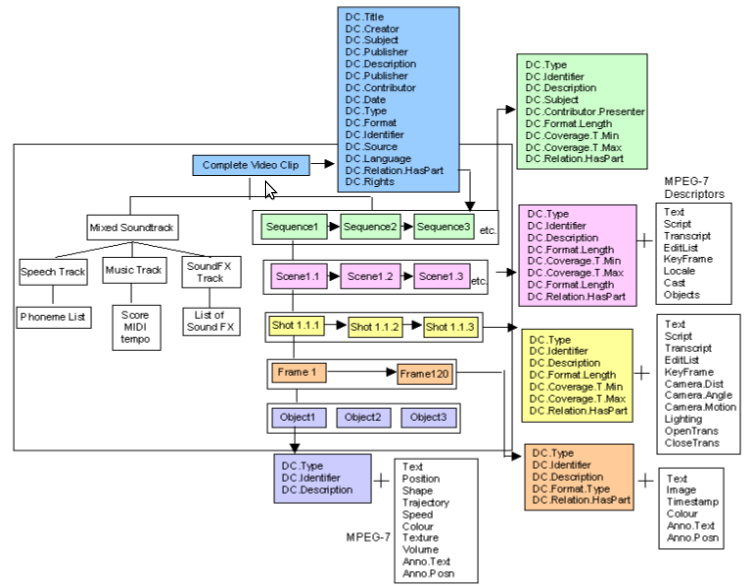
\includegraphics[width=0.8\textwidth]{images/HunterDCMI-MPEG7.png}
\caption{Modèle de Dublin Core étendu pour l'audiovisuel avec des descripteurs MPEG-7 (\cite{Hunter1999})}
\label{img:dcmi-mpeg7}
\end{figure}


\paragraph{Application à l'audiovisuel}
La modélisation du DCMI Metadata Terms s'intéresse à la description de tout type de ressources sur le Web (ce qui est identifié par une URI \cite{Berners-Lee1998}).
Cette perspective très générique lui permet de s'appliquer à de nombreux cas d'usages sans pour autant traiter leurs spécificités. 
Ainsi, dans le cas de l'audiovisuel il faudrait étendre ce schéma pour décrire par exemple le format d'image, les différents contributeurs, inclure de nouveaux types de dates, de nouvelles classes de Termes etc.

\cite{Hunter1998} ont proposé une extension qui raffine les propriétés du Dublin Core et les applique à différents niveaux de composition de l'objet audiovisuel, voire la Figure \ref{img:dcmi-mpeg7}.
Ainsi, l'objet audiovisuel est d'abord décomposé en élément audio (avec des pistes de paroles, de musique et d'effets) et vidéo.
Puis la vidéo est hiérarchisée en séquences, scènes, plans, images et objets dans une image.
À chaque niveau s'applique un ensemble de propriétés, dont des ajouts par rapport au schéma (la Description est liée à une liste de Genre, le Format permet d'indiquer le diffuseur).
\cite{Hunter1999} poursuivent ce travail et propose une représentation de ce schéma pouvant être intégré à MPEG-7. 


\paragraph{Discussion}
L'approche poursuivie par \citeauthor{Hunter1999} est cependant assez contraignante du fait de la décomposition hiérarchique figée et non applicable à tous les types de production audiovisuelle.
En particulier, la notion de séquence et de scène est propre à la production de fiction. 
Les niveaux de hiérarchisation devraient s'adapter aux particularités de chaque type de production. 
De plus, la description des niveaux de fragmentation inférieurs à la séquence repose de plus en plus sur des descripteurs de MPEG-7. 
En effet, le nombre de propriétés de Dublin Core utilisées baisse à chaque niveau de fragmention et on n'utilise plus que trois propriétés pour le dernier niveau (\e{identifier}, \e{type} et \e{description} pour associer les descripteurs MPEG-7).
Ce déséquilibre progressif entre les deux schémas reflète bien leur cadre d'usage. 
Si Dublin Core est particulièrement pertinent pour les niveaux documentaires les plus hauts, sa pertinence diminue quand on rentre dans le détails des fragments audiovisuels.
Il est alors nécessaire de lui adjoindre un schéma de description propre à l'audiovisuel comme MPEG-7.
Finalement, un schéma comme DMS-1 (voir \ref{sec:wrapper}) apparaît comme plus adapté qu'une extension de Dublin Core + MPEG-7 pour couvrir ces besoins.
Et ce, d'autant plus, que DMS-1 fournit des informations plus adaptées à l'audiovisuel (ne serait-ce que l'exemple des titres) et favorise un découpage factuel extensible ainsi qu'une description éditoriale.



%=============
% \subsection{Modèles de description multimédia \e{a posteriori}}
\subsubsection{MPEG-7 : Multimedia Description Scheme}\label{sec:mpeg7}
% \cite{Hunter2001} ; \cite{Troncy2007} ; \cite{Nack2005a} ; \cite{Dasiopoulou2009} ; \cite{Garci$\delta_2$005} ; 

% à revoir
Parmi les normes utilisés pour décrire les contenus audiovisuels, MPEG-7 est certainement devenu le standard de l'industrie. 
Développé à partir de 1998 par le comité MPEG (Moving Picture Expert Group) à la suite des standards MPEG-1, MPEG-2 (norme de compression du signal audiovisuel) et MPEG-4 (norme de d'encodage multimédia basée sur les objets), MPEG-7 est devenu une norme ISO/IEC en 2001 puis mise à jour jusqu'en 2006. 

La norme définit un ensemble de \e{Descripteurs} (Descriptors, Ds) dont les valeurs permettent de caractériser un objet audiovisuel, qu'il s'agisse de composantes du signal ou bien d'autres aspects comme des informations relatives à sa création, sa structure, son usage passé et futurs etc.
Ces Descripteurs sont organisés en \e{Schémas de Descriptions} (Description Schemas, DSs) dont on peut avoir une vue d'ensemble dans la Figure \ref{img:soa:mds}.
C'est cette partie de la norme (\cite[Part 5 : Multimedia Description Scheme]{ISO/IEC2003}) que nous traiterons en particulier dans cette section. 

\begin{figure}[ht!]
\centering
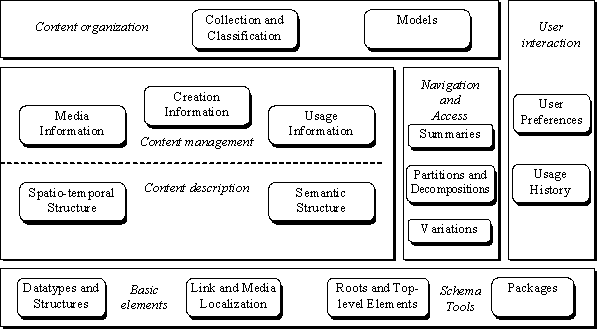
\includegraphics[width=0.8\textwidth]{images/MPEG-7-MDS.png}
\caption{Vue d'ensemble des Schémas de Description (DSs) de la norme MPEG-7}
\label{img:soa:mds}
\end{figure}

Les descriptions produites sont représentées dans un \e{Langage de Description des Définitions} (Description Definition Language, DLL) qui permet de spécifier la syntaxe des Descripteurs, la structure des Schémas de Description ainsi que la sémantique de l'ensemble.
Ce langage permet également de créer ou modifier des Descripteurs, d'étendre ou de modifier les Schémas de Descriptions. 
Le DLL est en réalité XML Schema (\cite{Fallside2004}) agrémenté de quelques types primitifs.

Pour utiliser MPEG-7, il faut également des outils et des directives annexes qui permettent de guider les utilisateurs. 
% définition / implémentation ? 
Dans la partie \e{Systems} de la norme, on trouve ainsi la définition d'outils qui remplissent les fonctions suivantes : codage d'une description MPEG-7 en binaire ; mécanismes de transmissions des descriptions (en binaire ou en texte) à part ou en parallèle du contenu audiovisuel décrit ;  synchronisation entre description et contenu audiovisuel ; gestion des descriptions et de la propriété intellectuelle. 
La partie \e{Reference Software} présente des logiciels de références pour utiliser la norme.
Enfin, la partie \e{Conformance} explicite des directives et des procédures pour s'assurer de la conformité des descriptions produites.

Nous détaillerons dans la section suivante les Schémas de Description liés à la gestion du contenu (\e{Content Management} dans la Figure \ref{img:soa:mds}) et à la description du contenu (\e{Content Description}).\\


\subsubsection{MPEG-7 : Gestion du contenu}\label{sec:mpeg7-gc}
MPEG-7 définit trois concepts fondamentaux pour modéliser l'enregistrement d'une réalité en un contenu multimédia et les multiples transformations qu'il est possible de lui appliquer. 
Ainsi, pour chaque modalité d'enregistrement (audio, audiovisuel, photo etc.) MPEG-7 considère la création de trois éléments, une \pc{ContentEntity} (entité de contenu, CE), une \pc{MediaInstance} (instance de média, MI) et un \pc{MediaProfile} (profil de média, MP), voir la Figure \ref{img:soa:media}.
Pour donner une première idée, on peut dire que le fichier créé correspond à la \pc{MediaInstance}, que le \pc{MediaProfile} correspond aux paramétrages de son encodage et que la \pc{ContentEntity} représente le contenu de manière abstraite.

\begin{figure}[ht!]
\centering
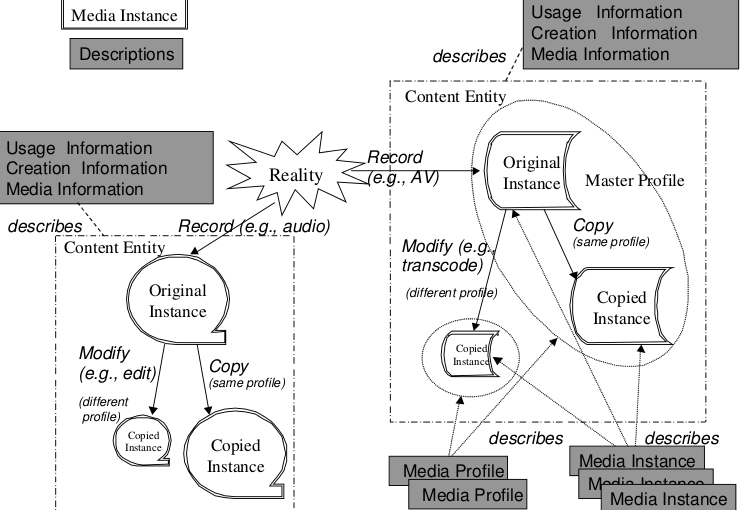
\includegraphics[width=0.8\textwidth]{images/MPEG-7-MediaManagement.png}
\caption{Gestion des contenus dans MPEG-7 à trois niveaux : contenu, instance et profile.}
\label{img:soa:media}
\end{figure}


On remarque qu'il existe cependant des différences dans les \pc{MediaInstance}, entre l'original et ce qui est nommé des \gui{copies} (copied instances). 
Ce qui est particulièrement intéressant pour nous est la constation que la nature de la manipulation entre l'original et les soi-disantes \gui{copies} importe peu (copie technique, réencodage ou montage), car cela crée de toute façon une nouvelle \pc{MediaInstance}. 
Le \pc{Variation DS} permet ainsi d'indiquer la nature de la variation entre les copies (résumé, traduction, changement de codage de la couleur etc. mais également une révision ou bien une version alternative pour le contenu).

À l'inverse, la notion de \pc{MediaProfile} est dépendante de la nature de ces transformations. 
Le \gui{MasterProfile} correspond ainsi aux paramètres d'encodage de la MI d'origine, la première créée. 
Ainsi, dès qu'une différence d'encodage apparaît avec les MI créées ultérieurement, un nouveau \pc{MediaProfile} est créé. 
Il correspond donc à un regroupement de toutes les instances ayant en commun le même encodage. 
%%%% orthographe %%%%
Ce qui paraît troublant néanmoins, est l'amalgame fait entre réencodage et montage. 
Les changements de structure réalisés par le montage semblent en effet bien plus significatif qu'un changement de paramètre d'enregistrement. 
On peut se souvenir de la citation d'\pc{Eisenstein} à ce sujet évoqué en \ref{sec:prod}.

Enfin, la notion de \pc{ContentEntity} correspond à une entité abstraite permettant de regrouper toutes les versions ultérieures de ce même contenu.
De ce fait, c'est à elle qu'on attache des informations concernant la création, l'usage et le type de média construit. % ??? Sûr ???
Ce regroupement d'informations à ce niveau découle de l'idée que chaque \pc{ContentEntity} définit une forme reconnaissable de contenu, quelque soit les variations apportées.
Encore une fois, l'idée qu'un montage différent n'impacte pas la forme et donc potentiellement l'identité du contenu nous semble ambiguë. 
Il s'agit là d'un de nos points d'achoppement par rapport à la modélisation proposée par la norme. 




\paragraph{Schémas de description}
Détaillons maintenant les trois Schémas de Descriptions proposés par MPEG-7 dans la partie \gui{Content Management}.
Remarquons que ces schémas s'appliquent tous à décrire les \pc{ContentEntity}.
% plus de détails sur les DSs

Le \pc{MediaInformation} est un schéma qui comporte des informations d'identification du CE ainsi qu'un ou plusieurs Profiles d'instances. 
Il faut remarquer que la définition du Profile proposée implique que le moindre changement d'encodage aboutit à la création d'un nouveau Profile en plus de l'instance. 
Il devient alors clair qu'un Profile représente la description d'un groupe d'instances, dont il facilite la gestion.
\begin{liste}
	\item \pc{MediaIdentification} : propose un ou plusieurs identifiants pour le CE.
	\item \pc{MediaProfile} : est composé de plusieurs descripteurs qui détaillent les paramètres et formats utilisés pour encoder une ou plusieurs instances.
	Il s'agit en particulier du \pc{MediaFormat} (pour l'encodage et le format d'encapsulation des données) ; le \pc{MediaInstance} (visant à identifier et localiser les instances) ; le \pc{MediaTranscodingHints} (pour faciliter le réencodage des données) ; le \pc{MediaQuality} (pour détailler la qualité et les défauts). 
\end{liste}


Le \pc{CreationInformation} peut être considéré comme une version étendue à l'audiovisuel des éléments du DCMI. Il comporte les Schémas de Description suivants : 
	\begin{liste}
		\item \pc{Creation} : des métadonnées qui permettent d'identifier le contenu (titre), proposer un résumé et des informations sur les conditions de sa création (créateur et contributeurs avec leur rôle, lieu, date, matériel et paramètrage utilisé).

		\item \pc{Classification} : des éléments de classification du contenu par forme (film, journal télévisé etc.), genre (sport, politique etc.), sujet, langage présent, et des informations sur la diffusion (date, région, public cible, critiques etc.)

		\item \pc{RelatedMaterial} : des métadonnées sur les autres versions d'un même contenu (format, type de média, localisation du média etc.) qui sont ensuite elles-mêmes décrites comme des éléments à part.
	\end{liste}



Le \pc{UsageDescription} est un schéma qui comporte un descripteur détaillant les droits attachés au contenu (\pc{Rights}), un descripteur décrivant les résultats financiers (\pc{FinancialResults}) et des schémas de descriptions sur les détails d'utilisation du contenu (\pc{Availability}) et sur l'historique de son utilisation(\pc{UsageRecord}).
Les droits d'exploitation peuvent en effet porter uniquement sur certains types de distribution (DVD, télédiffusion etc.) ou une certaine période. 
L'historique permet de garder une trace des diffusions et de leur audience.


\subsubsection{MPEG-7 : Description du contenu}\label{sec:mpeg7-dc}
\paragraph{La structure spatio-temporelle du contenu}
MPEG-7 fournit un ensemble de schémas et de descripteurs qui permettent de découper les contenus multimédias de toutes les manières possibles. 
Pour cela, la norme définit la notion de \pc{Segment} qui se décline en segment spatial, temporel ou spatio-temporel et sur tout type de média (audio, image, audiovisuel, multimédia). 
Chaque segment peut se décomposer en d'autres segments suivant la structure d'un arbre. 
De plus, ces segments peuvent être connectés entre eux ou pas, c'est-à-dire qu'ils peuvent spécifier trois zones d'une image (connexes ou pas) ou bien trois séquences temporelles (qui se suivent ou pas). 
Les Segments peuvent également n'être valables que pour une source média particulière, comme une piste audio comportant la musique.

Un point particulièrement important est que chacun de ces \pc{Segment} est considéré comme une \pc{ContentEntity}. 
On peut donc utiliser les schémas de \pc{MediaInformation}, \pc{CreationInformation} et de \pc{UsageDescription} pour les décrire ainsi qu'un schéma \pc{Semantic} que nous décrivons ci-après. 
En plus de cela, de nombreux schémas spécifiques à la nature du média existent pour décrire le signal de manière analytique. 


\paragraph{Aspects sémantiques}
Le schéma \pc{Semantic} permet de décrire le monde qui est présenté aux lecteurs dans le contenu audiovisuel. 
Il s'agit d'une description basée sur les évènements (\pc{Event}) ayant lieu à tel moment (\pc{SemanticTime}), à tel endroit (\pc{SemanticPlace}), et auxquels participent des objets (\pc{Object}) ou des agents (\pc{AgentObject}). 
La description peut être raffinée en utilisant des concepts (\pc{Concept}), en détaillant les attributs d'une entité (\pc{SemanticState}) ou bien les relations entre entités (\pc{SemanticRelation}).
À noter, que ces relations peuvent tout autant porter sur les évènements se déroulant dans le contenu (par exemple, l'agent A est bénéficiaire d'un évènement B) ou bien entre un contenu et des entités sémantiques (par exemple, l'image A est une référence à l'objet B).

% VariationDescription !!!!







%Core Ontology for MultiMedia
%=============
\subsubsection{Ontologies basées sur MPEG-7}\label{sec:mpeg7etc}
% \addcontentsline{toc}{subsubsection}{Core Ontology for MultiMedia}
MPEG-7 est une norme qui propose de nombreux descripteurs pour modéliser les objets audiovisuels.
La grande force de son approche est d'associer ces descripteurs à n'importe quelle séquence de contenu multimédia.
Cette richesse amène également une certaine difficulté dans l'appréhension de sa modélisation, tant la norme est étendue et complexe. 
De nombreux auteurs ont critiqué l'approche de représentation de la norme, notamment du fait de l'ambiguïté sémantique et syntaxique des descriptions produites (\cite{VanOssenbruggen2004, Nack2005a, Troncy2007, Dasiopoulou2009, Arndt2007}).

En effet, si l'utilisation des langages XML semblait légitime à l'époque, il en résulte un manque de formalisation qui complique les raisonnements et l'interopérabilité avec d'autres schémas de description (\cite{Nack2005a}).
De plus, la possibilité de créer plusieurs variantes syntaxiques valides pour représenter la même description rend difficile leur maintien et leur intéropérabilité, et ce même avec d'autres descriptions MPEG-7 (\cite{Arndt2007}).
Une approche formalisée sémantiquement aurait permis de réconcilier ces différentes variantes de représentation. 

Deux autres inconvénients mis en évidence par \cite{Nack2005a} sont la rigidité structurelle des descriptions et l'abscence de relations entre documents. 
La description d'un fragment de contenu ne peut se faire hors d'une structure de description d'un document entier. 
Une fois cette structure fixée, elle ne pourra plus être altérée, sous peine de la rendre incompatible avec les anciennes versions.
Les relations doivent également être contenu à l'intérieur d'une description d'un document.
De ce fait, créer une relation entre deux programmes obligent à créer un document de type collection contenant ces deux programmes.

MPEG-7 reste une source de référence et d'inspiration pour plusieurs séries de travaux qui tentent de pallier ces défauts de représentation.
Leur approche consiste à proposer une formalisation sémantique d'une partie du standard avec pour objectif de relier ces descriptions à des ontologies de domaine.
\cite{Troncy2007} et \cite{Dasiopoulou2009} ont étudié plusieurs de ces travaux en vue de les comparer, voir la Table \ref{tab:ontos} pour une synthèse de leur comparaison. 
Dans la suite de la section, nous présentons chacun de ces travaux avant de faire le point sur leur stratégie respective d'intégration d'ontologies de domaine.
Enfin, nous discutons des apports et des manques de ces ontologies par rapport aux besoins que nous avons exprimés en début de chapitre (\ref{sec:bm-av}).
Ces travaux se distinguent de plusieurs manières : 
\begin{liste}
	\item Par l'étendue de leur reprise de \g{MPEG-7} (colonne éponyme).
	On remarquera en particulier que les ontologies construites se concentrent sur les parties de décomposition structurelle des objets audiovisuels (Structure), et sur les descripteurs bas-niveau (Visual DS et Audio DS).
	\item L'ontologie générique à laquelle se raccroche l'ontologie construite (colonne \g{Ontologie}) 
	\item La conceptualisation utilisée pour réaliser des alignements et des liens avec des ontologies de domaine (colonne \g{Intégration}) 
	\item Le domaine et le type d'applications visées (colonne \g{Applications}) 
	\item Le langage de représentation utilisé (RDF-S ou OWL) (colonne \g{Langage}) 
	\item Le type de modélisation, modulaire (fond blanc) ou monolithique (fond gris).
\end{liste}

\begin{table}[htb!]
% \begin{center}   			{l p{61pt} p{60pt} p{130pt} r}
							% {l p{55pt} p{35pt} p{55pt} p{130pt} r}
\begin{tabularx}{\textwidth}{|l|p{61pt}|X|X|p{130pt}|r|}
\hline
	\g{Nom} & \g{MPEG-7} & \multicolumn{2}{c|}{\g{Ontologie}~|~\g{Intégration}} & \g{Application} & \g{Langage} \\ \hline\hline
	
	\rowcolor{lightgray}
	\pc{Harmony} &  Structure+ Visual & \multicolumn{2}{>{\columncolor{lightgray}}c|}{ABC} & analyse et annotation d'image dans le milieu médical & OWL Full \\ \hline
	
	\pc{aceMedia} & Structure+ Visual& \multicolumn{2}{c|}{DOLCE Lite+ AO} & analyse et annotation de match de tennis & RDF-S \\ \hline

	\pc{SmartWeb} &  Structure+ Visual & \multicolumn{2}{c|}{SmartSUMO} & analyse et annotation de vidéo de match de football & OWL \\ \hline

	\pc{Boemie} & Structure+ Visual+Audio & -- & Boemie & analyse, annotation et recherche de documents multimédia & OWL-DL  \\ \hline
	
	\pc{COMM} & Structure+ Visual & \multicolumn{2}{c|}{DOLCE} & gestion de documents multimédia pour l'industrie & OWL-DL \\ \hline

	\rowcolor{lightgray}
	\pc{Rhizomik} & MPEG-7 en entier & -- & Semantic DS & conversion MPEG-7 XML vers OWL & OWL-DL \\ \hline

	\pc{DS-MIRF} & MDS complet & -- & Semantic DS & conversion MPEG-7 XML vers OWL (football et formule 1) & OWL-DL \\ \hline
\end{tabularx}
\caption{Synthèse des ontologies basées sur MPEG-7}\label{tab:ontos}
% \end{center}
\end{table}



\paragraph{\pc{Harmony}}
\cite{Hunter1999} ont réalisé la première tentative de formalisation sémantique de MPEG-7. 
L'ontologie \pc{Harmony} était représentée initialement en RDF-S puis en OWL Full, et suit de près la modélisation proposée par MPEG-7. 
Il en résulte les mêmes constats que pour MPEG-7 ; la modularité des descriptions ainsi qu'une ambiguïté syntaxique et sémantique.

Les travaux de \cite{Hunter2001} ont intégré l'ontologie générique ABC permettant de modéliser des temporalités (évènement, situation, action), des actualités (artefact ou agent) et des oeuvres.
L'intégration d'ABC doit aussi permettre de créer des relations ou des alignements avec des ontologies génériques ou de domaine, pour favoriser l'interopérabilité et la spécialisation des descriptions. 
\cite{Hunter2004} est un exemple d'utilisation de l'ontologie pour l'annotation et l'analyse d'images médicales. 


\paragraph{\pc{aceMedia}}
Le projet \pc{aceMedia}\footnote{http://www.acemedia.org} a développé deux ontologies basées sur MPEG-7. 
La \pc{Multimedia Structure Ontology} (MSO) pour la description de la structure des objets audiovisuels, et la \pc{Visual Descriptor Ontology} (VDO) pour les aspects visuels (\cite{Petridis2004, Martinez2002}).
Ces ontologies proposent une modélisation modulaire, proche de MPEG-7, mais qui clarifie certaines ambiguïtés syntaxiques, à l'inverse d'\pc{Harmony}.
Par exemple, MSO introduit les classes \cd{mso:Frame} et \cd{mso:KeyFrame} afin de distinguer leur rôle respectif. 
Dans MPEG-7 et \pc{Harmony}, la description d'une image pouvait résulter de l'utilisation d'un \pc{VideoSegment} ou d'une \pc{StillRegion}.

MSO et VSO utilisent deux ontologies génériques, DOLCE Lite et l'Annotation Ontology (AO).
L'AO a été construite pour spécialiser les entités de DOLCE (\cite{Borgo2002}) afin de faciliter la mise en relation avec des ontologies de domaine.
Ces ontologies ont été utilisées pour l'analyse et l'annotation d'images et de vidéos dans le domaine du sport (jeu de tennis, \cite{Petridis2006}) et pour des vidéos personnelles.


\paragraph{\pc{SmartWeb}}
Le projet \pc{SmartWeb}\footnote{http://www.smartweb-projekt.de/start\_en.html} a permis de développer un ensemble d'ontologies pour construire des services d'in\-fo\-rmation sur le Web. 
Parmi cet ensemble, on trouve une ontologie d'annotation de contenu multimédia qui se construit sur l'ontologie générique SmartSUMO (\cite{Oberle2007, Vembu2006}).
SmartSUMO est elle-même développée dans ce projet à partir de DOLCE (\cite{Borgo2002}) et SUMO (\cite{Niles2001}). 
Par rapport aux deux premières ontologies, celle-ci permet d'ajouter des informations de création et de production en formalisant le processus d'annotation lui-même.

Une particularité de la modélisation est de considérer les objets multimédia et les segments comme deux classes soeurs, et non comme une spécialisation, ce qui amène certaines ambiguïtés dans des décompositions complexes.
L'ontologie a été utilisée pour l'analyse et l'annotation de vidéos de match de football.


\paragraph{\pc{Boemie}}
Le projet \pc{Boemie}\footnote{http://www.boemie.org/} a permis de développer deux ontologies ; la \pc{Multimedia Content Ontology} (MCO) et la \pc{Multimedia Descriptors Ontology} (MDO). 
Ces ontologies visent à re-modéliser MPEG-7 en OWL-DL, du point de vue de la décomposition des objets audiovisuels et des descripteurs audio et vidéo de bas-niveau (\cite{Dasiopoulou2009a}).

On retrouve la séparation entre objets audiovisuels et segments, mais cette modélisation utilise des restrictions de classes pour éviter toute ambiguïté.
La décomposition peut également se faire de manière indépendante sur un plan logique (unité logique) et factuel (segments).
Le lien avec des ontologies de domaine se fait par des relations pointant vers des concepts génériques de MCO.
\cite{Karkaletsis2005} proposent une utilisation de ces ontologies dans le cadre de l'analyse, l'annotation et la recherche de documents multimédia.


\paragraph{COMM}
La \pc{Core Ontology for MultiMedia} (COMM) est la tentative la plus récente de formalisation de MPEG-7 (\cite{Arndt2007, Staab2008, Arndt2009}).
Ce travail permet de spécialiser au domaine de l'audiovisuel les patrons de conception (Design Pattern) suivants : \pc{Descriptions \& Situations} (D\&S) et \pc{Ontology of Information Objects} (OIO) de DOLCE (\cite{Gangemi2005}).
COMM retravaille la modélisation de MPEG-7 pour la formaliser et la rendre modulaire. 

COMM définit 4 patrons ; la \e{décomposition structurelle} d'un objet en segments multimédia ; l'\e{annotation de contenu} qui permet d'associer des informations à un objet ou un segment ; l'\e{annotation du média} qui décrit les fichiers multimédias, leur encodage etc. ; l'\e{annotation sémantique} qui permet d'associer les objets ou segments multimédias avec des éléments d'ontologies de domaine. 
Une des particularités de COMM est de formaliser le processus d'annotation, mais pas tout à fait de la même manière que les ontologies de \pc{SmartWeb}.
L'annotation est ici le résultat d'une méthode d'annotation (manuelle, automatique), dont on peut décrire les paramètres, et qui sert de lien entre l'élément annoté et l'annotation sémantique.

L'ontolgoie COMM a été utilisée pour la gestion de documents multimédia dans des applications industrielles (comparateur de voitures, gestion de problèmes moteur pour l'aéronautique).
Si COMM clarifie la modélisation de MPEG-7, l'utilisation de DOLCE tend également à la complexifier.
Ainsi, une API\footnote{http://multimedia.semanticweb.org/COMM/api} Java a été développée pour cacher cette complexité et faciliter la création de descriptions et l'implémentation de services de recherche.



\paragraph{\pc{Rhizomik}}
Contrairement aux approches précédentes, \cite{Garcia2005} ont developpé une méthode de conversion automatique de MPEG-7 dans le cadre du projet \pc{ReDeFer}\footnote{http://rhizomik.net/redefer}.
Alors que les autres approches retravaillent la modélisation de MPEG-7 pour la clarifier et l'ajuster à leurs besoins, cette méthode reprend directement le XML Schema du standard.
La méthode repose sur deux langages d'alignement, XML2RDF et XML2OWL qui permettent de convertir tous les éléments en une ontologie OWL nommée \pc{Rhizomik}.

La séparation entre objets et segments multimédia est totale puisque les deux classes ne sont même pas soeurs.
De plus, reprenant MPEG-7, cette nouvelle représentation conserve les défauts déjà mentionnés : ambiguïté et complexité.
Du point de vue de la mise en relation avec des ontologies de domaine, cela est rendu possible par l'intermédiaire du Semantic DS.
Cette modélisation (décrite en \ref{sec:mpeg7}) est plus orientée et moins complète que celle proposée par des ontologies génériques.
De plus, l'approche nécessite d'utiliser un XML Schema pour définir les concepts du domaine, avant de pouvoir effectuer la transformation en une ontologie OWL.
De ce fait, l'ontologie est mieux utilisée pour transformer des descriptions MPEG-7 que pour faciliter l'intégration avec d'autres ontologies.


\paragraph{DS-MIRF}
\cite{Tsinaraki2004a, Tsinaraki2007} présentent le DS-MIRF framework qui traduit manuellement le MDS, l'Audio DS et le Visual DS en une ontologie OWL-DL.
Plus précisément, la transformation est pilotée par une ontologie tierce qui définit les alignements en XML Schema et les entités OWL.
Cette méthode permet d'expliciter et de clarifier certaines ambiguïtés de MPEG-7, mais la structure de l'ontologie reste proche de celle de \pc{Rhizomik}.

Une méthodologie a été proposée pour traduire systématiquement les déclarations réalisées avec une ontologie de domaine en déclarations compatibles avec la sémantique de MPEG-7.
Ainsi, contraiment à la méthode de \pc{Rhizomik}, l'intégration avec d'autres ontologies est réalisé en définissant un alignement, plutôt qu'en transformant les ontologies en XML Schema.
Le DS-MIRF framework a été utilisé pour l'annotation de match de football et de courses de Formule 1.


\paragraph{Stratégies d'intégration à des ontologies de domaine}\label{sec:strats-domaine}
En guise de synthèse, nous comparons les stratégies d'intégration des ontologies basées sur MPEG-7 avec des ontologies de domaine.
Ces ontologies de domaine servent à produire des descriptions sur le contenu d'objets ou segments multimédia, en proposant des concepts et des propriétés spécifiques à ce domaine. 
Nous avons vu que de nombreux exemples d'applications s'intéressent à un domaine sportif (football, tennis etc.).
Cela permet alors d'enrichir la description, essentiellement technique, de ces objets et de proposer une indexation propre à un métier.
Dans notre cas, l'enrichissement souhaité serait d'intégrer les connaissances fabriquées par les contributeurs de la chaîne de production.
Les ontologies présentées mobilisent trois stratégies : 
\begin{liste}
	\item \e{l'utilisation d'une ontologie générique} pour faire le lien entre les objets multimédia et des descriptions issues de l'ontologie de domaine. 
	C'est le cas de l'ontologie \pc{Harmony} avec ABC, des ontologies du projet \pc{aceMedia} et \pc{Boemie}.
	L'ontologie générique fournit des classes génériques que l'ontologie multimédia et de domaine peuvent spécialiser. 
	Ces classes sont reliées par des propriétés génériques, et spécialisables, qui permettent de relier un objet multimédia avec des déclarations de l'ontologie de domaine.
	Dans ce cas, l'intégration entre les ontologies dépend fortement de l'architecture de l'ontologie générique.

	\item \e{l'utilisation du Semantic DS}, moins complet et plus orienté que les ontologies génériques.
	C'est le cas des ontologies \pc{Rhizomik} et DS-MIRF, même si elles n'utilisent pas tout à fait la même méthodologie (voir leur présentation) pour faire l'intégration.

	\item \e{une formalisation de la méthode de création des liens} en plus de la formalisation des liens entre objets multimédia et descriptions sémantiques. 
	C'est l'approche utilisée dans COMM et les ontologies de \pc{SmartWeb}.
\end{liste}

Enfin, il est important de noter que dans les approches utilisant des ontologies génériques, la modélisation des objets audiovisuels est indépendante de la stratégie d'intégration à des ontologies de domaine.
Ainsi, il serait possible d'utiliser la dernière approche dans \pc{Harmony}.

\paragraph{Discussion}
Concernant la modélisation des objets audiovisuels, MPEG-7 et les ontologies réutilisant le Structure DS décomposent très finement le matériel audiovisuel dans l'espace et le temps [\g{$\chi_1$ : autonomie}].
Les \pc{Segments} ainsi constitués renvoient alors au premier des trois niveaux de modélisation de MPEG-7, à savoir \pc{ContentEntity} (CE), \pc{MediaProfile} (MP) et \pc{MediaInstance} (MI).
Cette modélisation en niveaux permet d'identifier les variations construites à partir d'un même matériel audiovisuel, de les regrouper et d'associer la plupart des informations au niveau supérieur (CE).
Ainsi, un CE peut regrouper plusieurs MP qui correspondent à un profil de transformation qui rassemble lui-même toutes les occurrences (MI) correspondant à ce profil.
Une critique importante de ce système est de ne pas distinguer entre la nature des transformations effectuées sur le matériel original, et en particulier entre une transformation d'encodage et de montage.

Ainsi, le CE vise plus à rassembler les informations communes à plusieurs variations de matériels audiovisuels que de modéliser un document ou un fragment documentaire portant une intention spécifique (voir la définition du document numérique section \ref{sec:docnum}).
De même, un MP et ses MI visent simplement à identifier et gérer des variations d'un même matériel, sans pour autant le raccorder à un projet documentaire en construction.
Les décompositions ou bien les variations identifiées avec MPEG-7 ne correspondent pas a priori à celles utilisées pendant la production pour organiser le travail ou bien sa présentation (structure documentaire auctoriale, voir \ref{sec:uc-sd}).
Or l'identification de cette structure première semble pourtant décisive quand il s'agit de réutiliser des fragments de documents dans de nouveaux contextes d'exploitation. 
De notre point de vue, il ne suffit pas d'identifier des segments ou des variations pour les constituer comme des fragments automones s'intégrant à un document audiovisuel.

En particulier, il peut être important de spécifier la grammaire documentaire d'un genre de document pour faciliter les manipulations de ses fragments. 
De ce point de vue, MPEG-7 définit une classification par genre et permet de typer les \pc{Segments} suivant leur place dans la structure de présentation du contenu.
Ces classifications peuvent être étendues par les utilisateurs mais aucune contrainte de composition n'est prévue, empêchant la modélisation d'une grammaire.
L'usage de ces classifications par unité de présentation vise à faciliter le travail d'analyse du signal, notamment la reconnaissance optique des caractères (ROC).
On retrouve ainsi l'esprit général de la norme qui consiste à opérer des décompositions a posteriori sur le matériel, et non à repérer des fragments documentaires qui ont porté l'intentionnalité de leur auteur pendant la production du document.
Ainsi, on peut dire que MPEG-7 vise plus à documenter l'analyse, que la production audiovisuelle.\\


En tant que CE, chacun des \pc{Segment} d'une décomposition peut-être décrit par les schémas de descriptions et le schéma Semantic DS [\g{$\chi_2$ : réutilisabilité}].
MPEG-7 proposent de nombreux descripteurs du matériel audio-visuel ainsi que des métadonnées sur le contexte de production.
Cependant, ces métadonnées ne permettent pas de rendre compte de l'organisation de la production, des résultats intermédiaires produits, ainsi que des connaissances fabriquées. 
Même si ces informations peuvent être associées à n'importe quel \pc{Segment}, il s'agit plus d'annoter l'objet audiovisuel fini, plutôt que de rendre compte de sa production.
Les descripteurs, quant à eux, renseignent sur les caractéristiques du matériel en tant que signal (à encoder, à transmettre etc.) à partir duquel des algorithmes cherchent à reconnaître des objets signifiants.
La reconnaissance automatique est une première étape, qui doit conduire à un étiquettage selon une sémantique propre à un contexte d'usage (une tâche et des utilisateurs).
Dans le cas de MPEG-7, nous n'avons pas observé de système capable de fournir des connaissances liées à la production audiovisuelle, mais sur d'autres domaines comme le sport ou la médecine.

Le schéma \pc{Semantic} esquisse une description visant des entités représentées dans le matériel audiovisuel (objet, évènement, lieux, agent) et esquisse ainsi une ouverture à des descriptions propres à un domaine.
Les ontologies basées sur MPEG-7 s'attaquent largement à cette question avec diverses stratégies (voir \ref{sec:strats-domaine}). 
Les stratégies de \pc{SmartWeb} et COMM consistant à modéliser la création de liens entre objets multimédias et connaissances d'un domaine sont les mieux formalisées et les plus génériques.
Cette généricité, qui vient de l'intégration du module OIO de l'ontologie DOLCE, rend leur appropriation plus difficile par rapport à des approches favorisant l'intégration d'une partie d'ontologie générique ou bien d'une ontologie noyau.
Il s'agit en quelque sorte de discuter du point de départ pour la construction d'ontologie avec l'alternative classique de \ciel{coller au problème, ou y plaquer un modèle} \parcite{Bachimont2004}.
L'approche \e{ascendante} se concentre sur la modélisation du problème, quitte à le rendre trop complexe pour être opérationnalisé, alors que l'approche \e{descendante} tente d'appliquer un schéma conceptuel générique aux spécificités du problème.





%=============
\subsubsection{Ontology for Media Resources}\label{sec:omr}
Suite aux travaux du W3C Media Annotation Working Group (MAWG), \cite{Burger2011} puis \cite{Lee2012} ont développé une ontologie minimaliste pour décrire et rechercher des informations sur des ressources média sur le Web.

\begin{figure}[ht!]
\centering
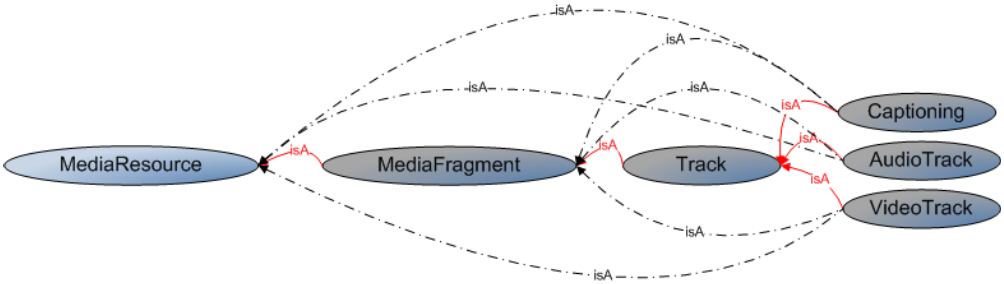
\includegraphics[width=0.8\textwidth]{images/MA-model.png}
\caption{Hiérarchie de classes sous le concept de \pc{MediaResource}}
\label{img:ma-model}
\end{figure}

La modélisation repose sur les concepts de \pc{Collection}, \pc{MediaResource}, \pc{MediaFragment}, \pc{Track} et \pc{Image}, voir la Figure \ref{img:ma-model}.
La décomposition des objets multimédia se fait donc par des fragments, que l'on peut ensuite décomposer en pistes et en images.
Cette simplicité apparente, comparée aux approches de segmentation complexe de MPEG-7, cache en réalité l'utilisation d'une autre recommandation du W3C.
La définition d'un MediaFragment peut se faire à partir de l'URI de son média source, où l'on ajoute un syntaxe de décomposition (\cite{Hausenblas2011}).
Par exemple, l'url suivante \cd{http://www.example.com/example.ogv\#t=10,20} désigne le fragment temporel commençant à 10s. et finissant à 20s.
La décomposition peut se faire selon une dimension spatiale, temporelle, en pointant une piste de la source, en pointant un autre fragment prélablement identifié, ou bien n'importe quelle combinaison de ces dimensions.
Des informations techniques (encodage, durée, format etc.) peuvent également être associées aux ressources.

En plus de ces classes, on trouve dans l'ontologie le concept d'\pc{Agent} (personne ou organisation), de \pc{Location} (lieu), de \pc{Genre} (le genre de programme suivant un dictionnaire spécialisé), de \pc{Rating} (permettant d'enregistrer les évaluations de lecteurs/spectateurs) et de \pc{TargetAudience} (indiquant le public visé par la ressource).
Ces classes supplémentaires permettent d'ajouter des informations sur le contexte de création (qui a participé, où) et de faciliter la diffusion et la recherche de ressource (genre, note, public cible etc.).

\begin{figure}[ht!]
\centering
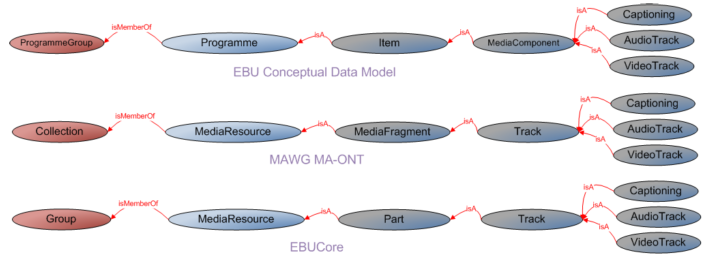
\includegraphics[width=\textwidth]{images/MA-alignement-A.png}
\caption{Alignement avec des ontologies multimédia (partie 1)}
\label{img:ma-alignement-A}
\end{figure}

\paragraph{Alignement avec d'autres conceptualisations}
Un apport important de cette ontologie réside dans le travail d'alignement avec les autres modélisations multimédia. 
Les Figures \ref{img:ma-alignement-A} et \ref{img:ma-alignement-B} présentent un alignement minimaliste des principales classes de l'\pc{Ontology for Media Resource}.
Dans la définition de \cite{Lee2012}, les alignements sont étendus à d'autres conceptualisations ainsi qu'aux propriétés de schémas de métadonnées et métadonnées embarquées dans des formats conteneurs.
Ainsi, on se rend compte que ces classes principales, qui représentent une collection d'objets multimédia, un objet, ses fragments et ses pistes de contenu, se retrouvent dans toutes ces modélisations. 
Les variations se situent à la fois dans la manière de découper/segmenter cet objet en fragment (dimension spatiale, temporelle etc.), de le lier aux média et dans la manière et la nature des informations que l'on peut leur associer.

\begin{figure}[ht!]
\centering
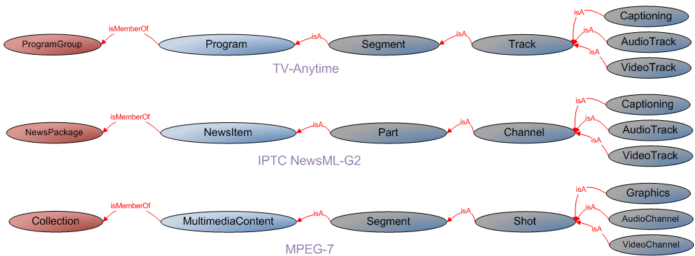
\includegraphics[width=\textwidth]{images/MA-alignement-B.png}
\caption{Alignement avec des ontologies multimédia (partie 2)}
\label{img:ma-alignement-B}
\end{figure}

\paragraph{Discussion}
L'\pc{Ontology for Media Resource} (OMR) a été construite dans un souci de clarté, de cohérence et d'extensibilité et s'intégre particulièrement bien avec les autres recommandations du W3C, dont le Media Fragment URI et SKOS.
L'objectif étant (1) de pouvoir publier des déclarations sur le web de données et (2) construire des systèmes de recherche de contenu interopérables. 
En effet, le travail réalisé sur les alignements permet d'extraire et traduire les informations contenues dans les dépôts n'utilisant pas les mêmes modèles.
Une API\footnote{http://www.w3.org/TR/2010/WD-mediaont-api-1.0-20100608/} a également été construite pour faciliter ces opérations et le déploiement de service de recherche et d'aggrégation de résultats provenant de ces différentes sources.

L'ontologie OMR ne se positionne donc pas comme un supplément de modélisation, mais plutôt comme un travail de synthèse et de mise en correspondance des travaux existants dans une représentation standardisée.
Son objectif n'est pas l'exhaustivité de la représentation des objets audiovisuels ou bien de leur description, mais bien de mettre en commun l'ensemble des informations dispersées et cloisonnées dans les dépôts.












% Our approach follows this trend of research with different focus and objectives than the works presented. We consider the shooting script as the main production document to describe the video shots. The focus is on the realization of these shots, not the preparation or direction of the production. It does not assist the same people and do not provide exactly the same pieces of information. As we demonstrated above, a Semantic Script can assist the cameraman at shooting time and the professional editor when reviewing. 
% In comparison to the COMM ontology, our model offers an additional representation layer with describe the editorial structure of audiovisual objects (Opus, MediaAsset, EditorialObject). With the Semantic Script, we provide a way to predefine a structure and capture intentions that are inherent to the audiovisual production process. COMM represents a MPEG-7 flavored description of video files and also the way this description has been produced by human or algorithms. This indexing is made after the video production and do not provide any mean to retain information from the context of production.


\subsection*{Discussion}
\addcontentsline{toc}{subsection}{Discussion}
La modélisation des objets audiovisuels que nous avons spécifiée dans notre cahier des charges (\ref{sec:cdc-av}) demande de distinguer les produits intermédiaires de la chaîne, afin de favoriser leur circulation et leur intégration dans d'autres chaînes de production [\g{$\chi_1$ : autonomie}].
Sur ce plan, MPEG-7 modélise les objets audiovisuels comme des matériaux audiovisuels que l'on décrit surtout selon des critères propres au signal et peu selon le point de vue de la production audiovisuelle.
La gestion de ces matériaux s'opère alors en fonction de leurs caractéristiques communes, différents niveaux permettant de les regrouper et de mettre en commun certaines informations. 
Ainsi , cette modélisation évacue largement les questions de construction documentaire pour se concentrer sur les stratégies de description exogènes.
Dans ce point de vue, toutes les transformations d'un matériel se valent, quelque soit l'effet sur le sens véhiculé par le segment audiovisuel. 
De même, le typage des segments ne permet pas de représenter des contraintes de structuration documentaire.
Les ontologies construites à partir de MPEG-7 partagent ces problèmes inhérents à l'approche de segmentation et de description de la norme.
L'alignement a minima des modèles de l'audiovisuel proposée en \ref{sec:omr} montre une relative homogénéité des concepts, ce qui tend à indiquer qu'ils partagent  ce manque de considération des problématiques documentaires. 

À l'inverse, les modèles de description \e{endogènes} que nous avons étudiés modélisent les objets audiovisuels en devenir, et décrivent justement la structure documentaire auctoriale qui guidera également la production du matériel audiovisuel.
Cette approche apparaît alors comme complémentaire par rapport aux modèles \e{exogènes}, dans le sens où la structure documentaire prévue devrait être associée et synchronisée au matériel audiovisuel effectivement produit.
On pourrait ainsi réaliser une modélisation dynamique de la production audiovisuelle.\\

% :  / gestion des variations d'un segment de matériel, plutôt que d'un fragment porteur d'une intentionalité et s'articulant dans une structure documentaire / se conformant à une grammaire de genre 
% => il n'y a pas de niveau documentaire, il n'y a pas de niveau de production ; il n'y a que du matériel dont on repère des ensembles cohérents suivant des critères techniques (transformé / même profil)

Les modèles de description \e{endogènes} mettent également en avant les connaissances mobilisées par les contributeurs de la chaîne de production [\g{$\chi_2$ : réutilisabilité}].
La description de la structure en devenir de l'objet audiovisuel permet ainsi d'associer d'autres connaissances à chaque fragment. Il s'agit par exemples de préciser la manière de les produire (indication de tournage, réglages d'équipement de captation etc.), ce qui se révèle particulièrement intéressant dans le cas de production collaborative.
MPEG-7, et les ontologies qui le formalisent, se concentrent sur une description du signal, tout en associant des informations éparses sur le contexte de production.
L'ouverture à une description sémantique présente dans MPEG-7 a été étendue dans certaines de ces ontologies afin de pouvoir intégrer des connaissances propres à un domaine.
Cependant, ces stratégies d'intégration sont difficiles à appréhender car reposant sur des ontologies génériques. 
Nous questionnons alors la pertinence de construire une ontologie noyau qui serait moins complète et plus centrée sur les problématiques de la production audiovisuelle collaborative.
% MPEG-7 : des md associant quelques valeurs au matériel produit, mais pas de description de sa production / pas de connaissances propre à la chaîne de prod., mais des descripteurs du signal / la représentation de MPEG-7 pose des problèmes sur le plan syntaxique et sémantique, les ontologies basées sur MPEG-7 s'attaquent à ces problèmes avec différentes stratégies / les formalismes permettant d'intégrer les connaissances d'un domaine sont difficile à appréhender, et on peut se demander s'il ne serait pas plus pertinent de construire une ontologie de noyau, moins complète et centré sur nos besoins 




% Along with MPEG-7, the MPEG-21 Multimedia Framework \cite{Burnett2003} offers a valuable perspective on future practices in content management, distribution and consumption. The recent interest in content value chains modeling presented in \cite{Garcia2010} shows some similarities with our audiovisual object modeling approach. There is still an open debate about the modeling of the various forms or facets that content can take during its production. Many approaches rely on, adapt or extend the original FRBR Group 1 concepts of \e{Work}, \e{Expression}, \e{Manifestation} and \e{Item}. 
% For instance, the Media Value Chain Ontology (MVCO) \cite{Rodriguez-Doncel2009}, \cite{Rodriguez-Doncel2010} is included as the Part 19 of the MPEG-21 standard. 
% The authors merge the concepts of Expression and Manifestation. Moreover, they also propose a new concept of Product for asset which needs to be licensed before publishing. 


% %=============
% \paragraph{TV Anytime}
% % \addcontentsline{toc}{subsubsection}{TV Anytime}
% \cite{Evain2000} ; \cite{Tsinaraki2004} ; \cite{Tsinaraki2005}

